\documentclass[12pt, a4paper]{article}
\usepackage[margin=1in]{geometry}
\usepackage{auxiliary/utilities/preamble}

\newcommand{\titulo}{Métodos de Runge-Kutta}

\begin{document}
\sffamily
\begin{titlepage}
    \begin{center}
        
\includegraphics[width=0.15\textwidth]{../auxiliary/assets/unam.png}
        \hspace{0.6\textwidth}
        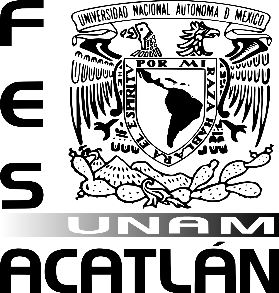
\includegraphics[width=0.15\textwidth]{../auxiliary/assets/fes.png}

        \vspace*{5cm}
        \LARGE
        \textbf{\titulo}

        \vspace{1cm}
        \large
        Camargo Badillo Luis Mauricio \\
        \vspace{1.5cm}

        \vfill

        \vspace{0.5cm}
        Audiciones Fase 3 \\
        \textbf{Programa de Inducción a Matemáticas Aplicadas y Computación}\\
    \end{center}
\end{titlepage}


\tableofcontents
\newpage

Recordemos que una \textit{ecuación diferencial} es una ecuación que relaciona una (o más) funciones con sus derivadas. Estas ecuaciones son de gran utilidad, pues nos ayudan a modelar muchos fenómenos naturales, el objeto de estudio de muchas disciplinas como la física, la ingeniería, la química, la biología, la astronomía, etc.; las ecuaciones diferenciales también modelan otros fenómenos de la economía y otras ciencias matemáticas. Es por esta razón por la que la resolución de ecuaciones diferenciales es un área de tanto interés en el mundo actual.

Usualmente, al tener una ecuación diferencial, el objetivo es encontrar la función (o las funciones) que la satisfagan. No obstante, dependiendo de la complejidad de la ecuación y de su forma, puede ser difícil o incluso imposible encontrar la solución exacta y explícita de forma analítica, un problema que se presenta sin importar si buscamos la solución manualmente o le asignamos la tarea a una computadora. De hecho, son bastantes las aplicaciones que involucran ecuaciones diferenciales cuya solución no se puede obtener de forma analítica; las ecuaciones que definen la forma del ala de un avión son un ejemplo.

Es por esta problemática por lo que nos apoyamos de los métodos numéricos para resolver este tipo de ecuaciones diferenciales. Recordemos que los métodos numéricos son técnicas que nos ayudan a aproximar procesos matemáticos y que se han vuelto especialmente populares luego del \textit{boom} en poder computacional que se ha experimentado en las últimas décadas; la resolución de esta clase de ecuaciones diferenciales son tan solo una de las muchas aplicaciones de los métodos numéricos.

Evidentemente, dada la naturaleza de los métodos numéricos, no tendremos una solución exacta como la analítica, pero ciertamente podemos tener una solución lo suficientemente cercana como para poder confiar en ella. En el mundo actual, podemos constatar que las soluciones obtenidas son perfectamente válidas: miles de aviones vuelan todos los días a pesar de que las ecuaciones que modelan la aerodinámica deben ser resueltas numéricamente.

Los \textbf{métodos de Runge-Kutta} son algunos de los métodos numéricos más ampliamente utilizados para la resolución de estas ecuaciones diferenciales. Estos métodos proporcionan soluciones más precisas que aquellas dadas por otros métodos numéricos más sencillos, como el método de Euler. A lo largo de este documento, se estará dando un panorama general de estos métodos, sus diferentes tipos y cómo utilizarlos, cerrando con una aplicación.

\section{Introducción a los Métodos de Runge-Kutta}

\section{Tipos de Métodos de Runge-Kutta}

\section{Aplicaciones de los Métodos de Runge-Kutta}

\section{Conclusión}

\end{document}
